\section{Motivational Example}
\label{sec:example}
\begin{figure*}
\begin{center}
\begin{tabular}[t!]{ccc}\hspace*{-15pt}
	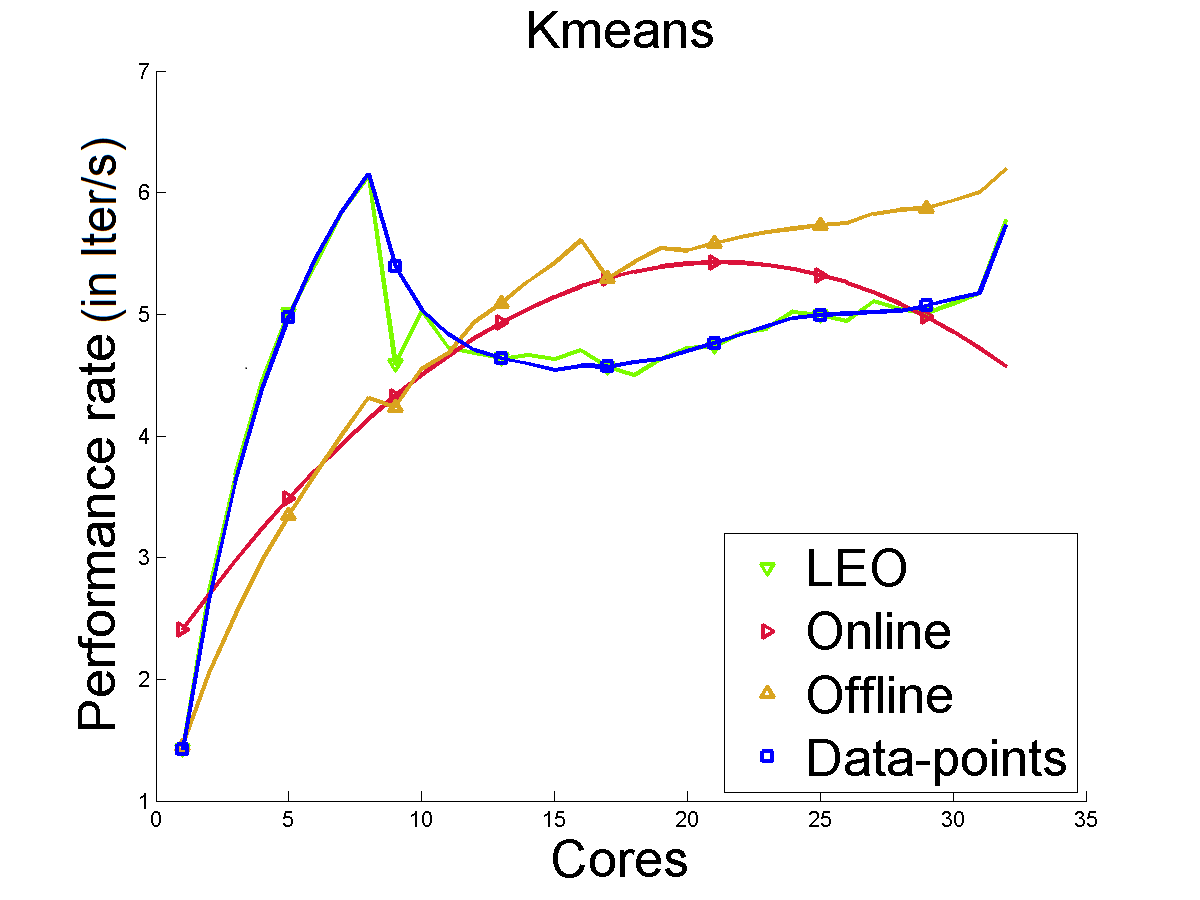
\includegraphics[width=0.3\textwidth]{KmeansCoresPerf.png}&
	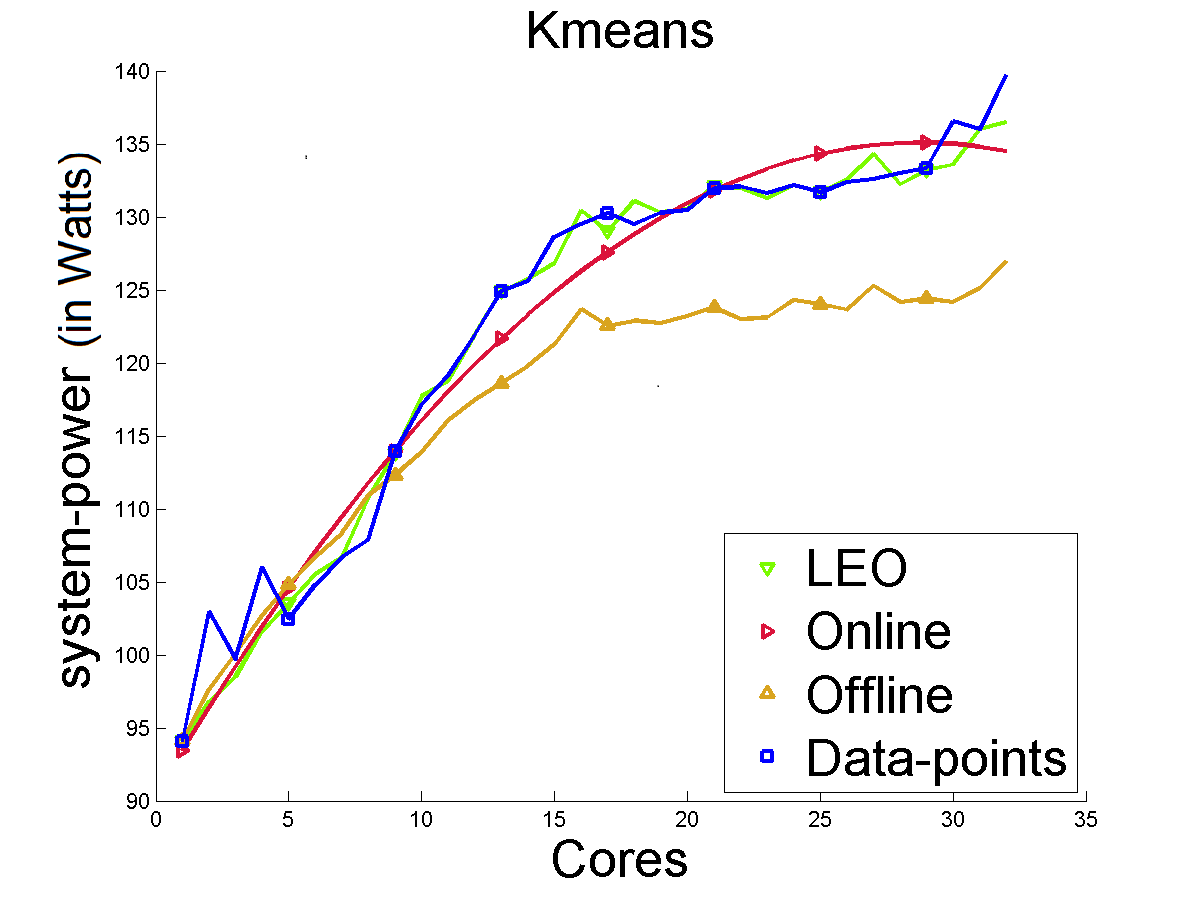
\includegraphics[width=0.3\textwidth]{KmeansCoresPower.png}&
	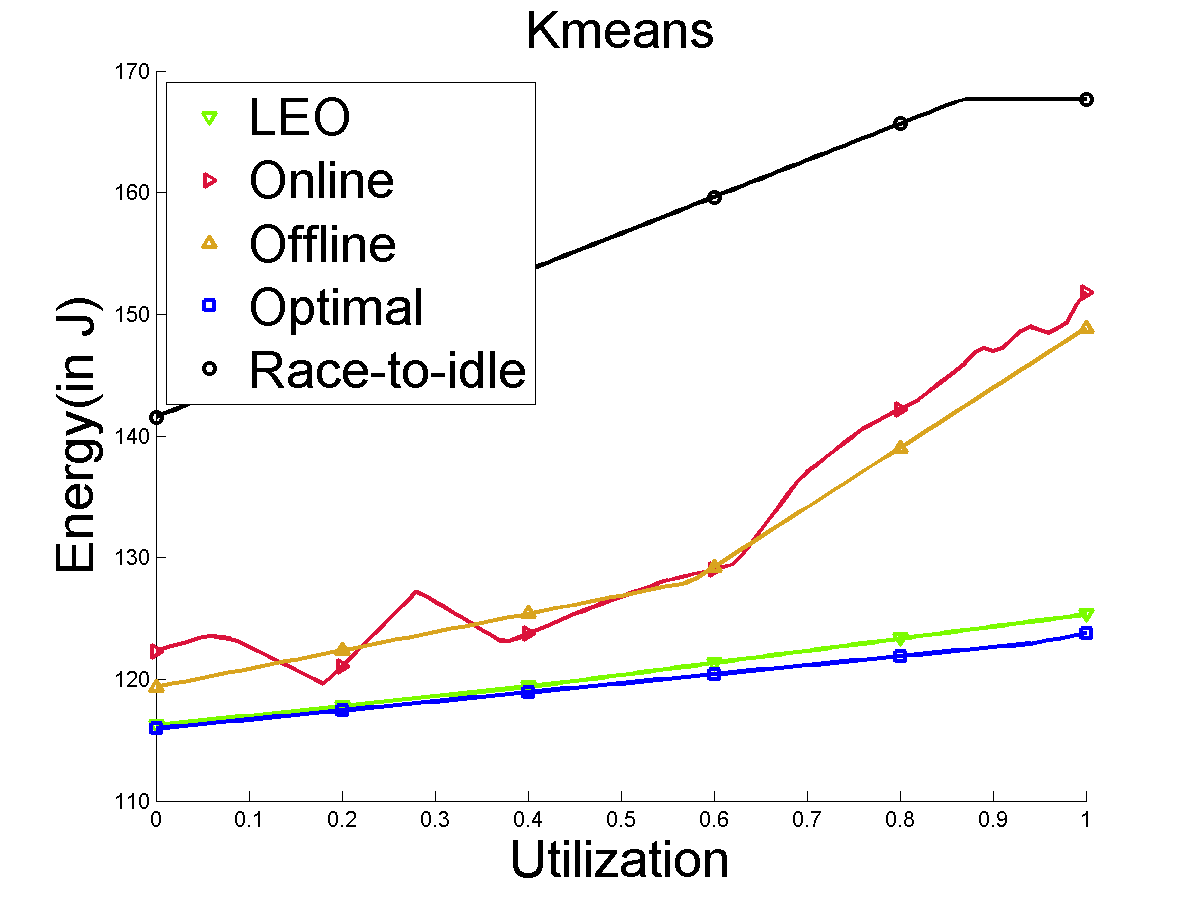
\includegraphics[width=0.3\textwidth]{KmeansCoresEnergy.png}\\
	 {(a)} &
	 {(b)} &
	  {(c)}
\end{tabular}
\vspace{-0.35em}
\caption{Power estimation for \texttt{Kmeans}
  clustering application using \SYSTEMLEO{}, \textit{Online} and
  \textit{Offline} algorithms. The estimations are made using only 6
  observed values (Cores) out of 32.\TODO{Add performance description}}
\label{fig:Kmeans}
\end{center}
\end{figure*}
\vspace{-0.35em} This section presents an example to motivate
\SYSTEMLEO{} and build intuition for the formal models presented
subsequently.  We consider energy optimization of the \texttt{Kmeans}
benchmark from Minebench \cite{minebench}.  Kmeans is a clustering
algorithm used to analyze large data sets.  For this example, we run
on a 16-core Linux x86 server with hyperthreading (allowing up to 32
cores to be allocated)\footnote{Our full system evaluation tests more
  parameters than simply core allocation.  See \Secref{sec:experiment}
  for details.}.  We assume that \texttt{Kmeans} may be run with
different performance demands and we would like to minimize energy for
any given performance demand.  To do so for \texttt{Kmeans} on our
32-core system we must estimate its performance and power as a
function of the number of cores allocated to the application.  Given
this information, we can easily select the most energy efficient
number of cores to use for any performance demand.

To illustrate the benefits of \SYSTEMLEO{}, we will compare it with three
other approaches: a heuristic, offline learning, and online learning.
The heuristic uses the well know \emph{race-to-idle} strategy --
simply allocating all resources (cores, clockspeed, etc.) to \texttt{Kmeans}
and then idling the system once the application completes.  The
offline learning approach builds a statistical model of performance
and power for each configuration based on prior measurements of other
applications.  The online approach uses polynomial regression to learn
the tradeoffs for each configuration while \texttt{Kmeans} is running. (More
details on the specifics of these approaches can be found in
\Secref{sec:poc}).

Each of these three approaches has their limitations.  The heuristic
approach simply assumes that the most energy efficient configuration
is the one where all the system resources are in use, but that has
been shown to be a poor assumption for this type of application
\cite{HotPower,MeisnerISCA2011}.  The offline approach predicts
average behavior for a range of applications, but it may be a poor
predictor of specific applications (\texttt{Kmeans}, in this case).  The online
approach will produce a good prediction if it takes a sufficient
number of samples, but the required number of samples may be
prohibitive.

\SYSTEMLEO{} combines the best features of both the offline and online
approaches.  At runtime, it changes core allocation (using process
affinity masks), observes the power and performance, and combines this
data with that from previously seen applications to obtain the most
probable estimates for other unobserved cores.  \PUNT{\SYSTEMLEO{}
  estimates \texttt{Kmeans}' power and performance in different configurations
  as a combination of both these online observations and prior
  observations from the similar applications.  Specifically,
\SYSTEMLEO{} observes only 6 separate allocations of cores to \texttt{Kmeans}.}
The key advantage of \SYSTEMLEO{}'s graphical model approach is
that it quickly finds similarities between \texttt{Kmeans} and previously
observed applications.  It builds its estimation not from every
previous application, but only those that exhibit similar performance
and power responses to core usage.  This exploitation of similarity is
the key to quickly producing a more accurate estimate than either
strictly online or offline approaches.

\PUNT{ It models the core count's effect on performance and power as a
  random variable drawn from a normal distribution where the mean and
  variance are unknown.  It then learns the \emph{covariance} matrix
  representing the similarity between these variables.  The entries in
  the covariance matrix will increase for applications whose power and
  performance are similar to \texttt{Kmeans} and decrease for those that are
  different.  So, when \SYSTEMLEO{} estimates power and performance for
  \texttt{Kmeans}, it does not use the priors for all applications, but instead
  just uses the ones that are most similar (have higher corresponding
  covariance).  Using this combination of online and offline
  approaches, \SYSTEMLEO{} quickly converges to highly accurate estimates
  of power and performance making it easy to solve the energy
  minimization problem.  }

\figref{fig:Kmeans} shows the results for this example.
\figref[a]{fig:Kmeans} shows each approach's performance estimates as
a function of cores, while \figref[b]{fig:Kmeans} shows the estimate
of power consumption.  These runtime estimates are then used to
determine the minimal energy configuration for various system
utilizations.  \figref[c]{fig:Kmeans} shows the energy consumption
data where higher utilizations mean more demanding performance
requirements.  As can be seen in the figures, \SYSTEMLEO{} is the only
estimation method that captures the true behavior of the application
and this results in significant energy savings across the full range
of utilizations.

Learning the performance for \texttt{Kmeans} is hard because the
application scales well to 8 cores, but its performance degrades
sharply with more.  It is quite challenging to find the peak without
exploring every possible number of cores. We observe the power and
performance at 6 uniformly distributed values (5, 10, $\cdots$, 30
cores).  The offline learning method predicts the highest performance
at 32 cores because that is the general trend over all applications.
The online method predicts peak performance at 24 cores, so it learns
that performance degrades, but requires many more samples to correctly
place the peak.  \SYSTEMLEO{} -- in contrast -- leverages its prior
knowledge of an application whose performance peaks with 8 cores.
Because \SYSTEMLEO{} has previously seen an application with similar
behavior, it is able to quickly realize that \texttt{Kmeans} follows
this pattern and \SYSTEMLEO{} produces accurate estimates with just a
small number of observations.

The next three sections formalize this example.  \Secref{sec:notation}
describes the notation we will use. \Secref{sec:problemFormulation}
presents a general formalization of this energy minimization problem
for any configurable system (not just cores).  \Secref{sec:HBN}
presents the technical description of how \SYSTEMLEO{} incorporates
online and offline approaches to find similar applications and produce
accurate runtime estimates of power and performance.
